\documentclass{article}
% packages
\usepackage {lmodern}
\usepackage [T1]{fontenc}
\usepackage {amsmath}
\usepackage {amssymb}
\usepackage {amsfonts}
\usepackage {graphicx}
\usepackage {fullpage}
\usepackage {gensymb}
\usepackage {caption}
\usepackage {subcaption}
\usepackage {array}
\newcolumntype{L}{>{\centering\arraybackslash}m{3cm}}
%\usepackage{nopageno}
\usepackage {cite}
\usepackage {setspace}
\usepackage [version=4]{mhchem}

% graphics path
\graphicspath {{images/}}


%begin document
\begin {document} 

\title { Determination of Water Hardness of Filtered and
Unfiltered Water using Complexometric Titration: \\ 
What Effect will a Brita\textsuperscript{\textregistered} Filter have on Water Hardness?}
\vspace{20cm} 
\author {Justin Chao - jc55395 
\\ Lab Partner: William Canales - wcc546 
\\ \\ CH 456} 

\maketitle

\newpage

\section {Introduction}
This experiment aims to determine the water hardness of a filtered and unfiltered water sample using
complexometric titration techniques.
Ethylenediaminetetraacetic Acid (EDTA) will be used as the complexing agent of choice.
Eriochrome Black T and Murexide will be used as complexometric indicators.

\subsection {Water Hardness}

Many domestic and industrial water users are concerned about the hardness of
their water. Hard water requires more synthetic detergents and soap for washing
and laundry, and contributes to scaling in industrial equipment and boilers.
The hardness of water is caused mainly by compounds of calcium and magnesium,
along with a variety of other metals. As water moves through soil and rock in
nature, its properties as an excellent solvent dissolves minute amounts of
minerals and keeps them in solution.

Due to the high concentrations of Ca$^{2+}$ and Mg$^{2+}$ ions usually found in
water, total water hardness is determined by the total concentrations of calcium
and magnesium ions. Calcium carbonate is the most common precipitate of hard
water, therefore total water hardness can be expressed as the CaCO$_3$ mg equivalent
to the total mass of calcium and magnesium measured in one liter of water.

Table 1 lists the different classifications of degrees of water hardness
according to the US Geological Survey. \cite{lab_man}

\begin{center}
        \captionof{table}{USGS classification of degrees of water hardness.}
        \begin{tabular}{|c|c|}
                \hline
                \textbf{Degree of Hardness} & \textbf{Measured Total Water
                Hardness (ppm CaCO$_3$)} \\
                \hline
                Soft & 0 - 60 \\
                Moderately Hard & 61 - 120 \\
                Hard & 121 - 180 \\
                Very Hard & > 181 \\
                \hline
        \end{tabular}
\end{center}


\subsection {Complexation Reactions}
Complexometric titrations are based on complexation reactions. These reactions consist of a
coordination complex being formed, consisting of a central atom or ion, which is usually metallic,
and a surrounding array of bound ions or molecules, known as complexing agents or ligands. A metal
complex is a coordination complex whose center consists of a metal atom. Figure 1 illustrates a metal
complex with a molybdenum central atom and CO and triphenylphosphine as ligands.

\begin{center}
    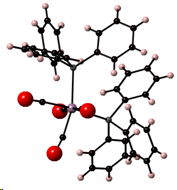
\includegraphics[scale = 0.6]{structurecis}
    \captionof{figure}{Structure of cis-[Mo(CO)$_4$(PPh$_3$)$_2$].\cite{ucla}}
\end{center}

A chelating ligand is one that can form several bonds to the metal ion. Such a ligand is also known
as a multidentate ligand.
Figure 2 illustrates the ligand dimethylgloxime as a chelating ligand against cobalt. There are
three geometries that can result from ligands chelating, or encapsulating, the central atom:
equatorial, facial, and cage.

\begin{center}
    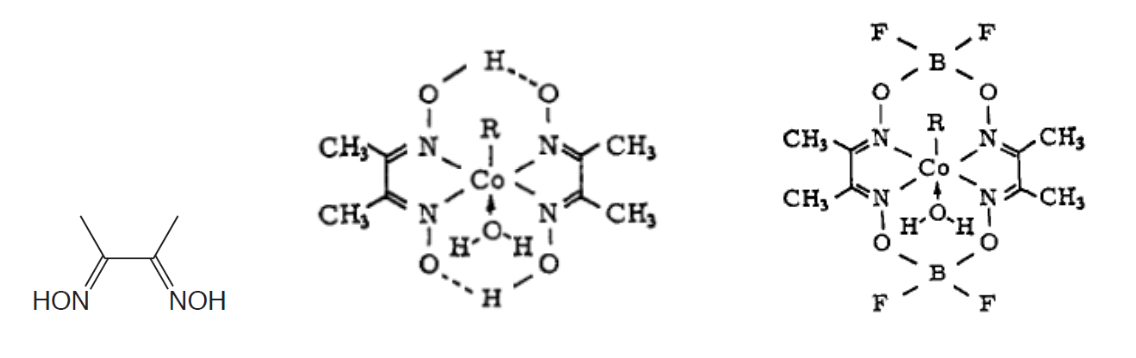
\includegraphics[scale=0.6]{struc}
    \captionof{figure}{left: The ligand dimethylglyoxime (dmgH), middle: a bis-ligated
        cobaloxime, right: a fluoroborated cobaloxime.\cite{schrauzer}}
\end{center}

\subsection{Ethylenediaminetetraacetic Acid (EDTA)}
In this experiment, EDTA will be used as a chelating agent against Ca$^{2+}$ and
Mg$^{2+}$.  EDTA, when fully protonated, is a weak acid and is often used in complexometric titrations
due to its ability to form stable and water-soluble complexes. EDTA also reacts
with most metal ions in a 1:1 stoichiometric ratio.  Figure 3 illustrates the
structure of EDTA and its complexation with a metal.


\begin{figure}[!hb]
\centering
        \begin{subfigure}{.5\textwidth}
        \centering
                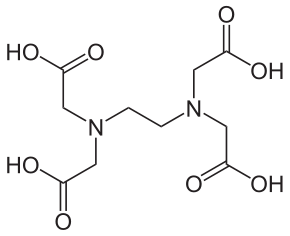
\includegraphics[width=.5\linewidth]{EDTA}
                \caption{Structure of EDTA}
                \label{fig:sub1}
        \end{subfigure}%
        \begin{subfigure}{.5\textwidth}
                \centering
                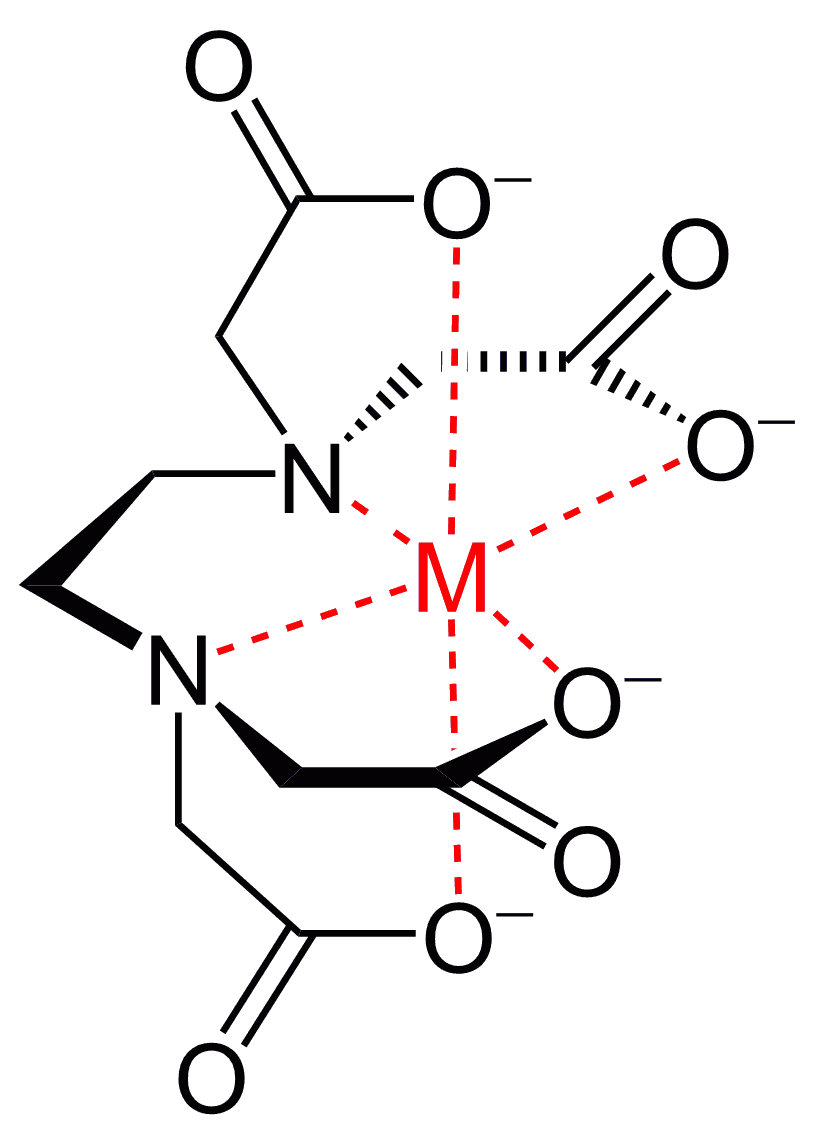
\includegraphics[width=.4\linewidth]{M_EDTA}
                \caption{Metal-EDTA chelate}
                \label{fig:sub2}
        \end{subfigure}
        \caption{Illustrations of EDTA as a chelating ligand.\cite{EDTA}}
\end{figure}

In this experiment, EDTA (or H$_6$Y$^{2+}$, where Y = C$_{10}$H$_{12}$N$_2$O$_8$) will be titrated
against a solution containing both Ca$^{2+}$ and Mg$^{2+}$ ions.  Of the various EDTA species, only
the Y$^{4-}$ ion complexes in a 1:1 ratio with metal ions.  Therefore, to increase the amount of
Y$^{4-}$, the pH of the solution is kept basic at around 10 using a buffer solution. \cite{mtsu}

Table 2 shows the different pK$_a$ values of EDTA. \cite{chemwiki}
\begin{center}
        \captionof{table}{Various pK$_{a}$ values of EDTA}
        \begin{tabular}{|c|c|c|c|c|c|c|}
                \hline
                & pK$_{a1}$ & pK$_{a2}$ & pK$_{a3}$ & pK$_{a4}$ & pK$_{a5}$ &
                pK$_{a6}$ \\
                \hline
                Values: & 0.0 & 1.5 & 2.0 & 2.66 & 6.16 & 10.24 \\
                \hline
        \end{tabular}
\end{center}
The first four pK$_a$ values correspond with the carboxylic acid protons, and
the last two values correspond with the ammonium protons.

While EDTA forms stable complexes with both Ca$^{2+}$ and Mg$^{2+}$, EDTA has a higher affinity for
calcium, and therefore will bind first to Ca$^{2+}$, resulting in the following reaction order:

\begin{center}
        \begin{align}
                \ce {Ca^2+ + Y^4- &-> CaY^2-}\\
                \ce {Mg^2+ + Y^4- &-> MgY^2-}\\
                \ce {Ca^2+ + MgY^2- &-> CaY^2- + Mg^2+}
        \end{align}
\end{center}

Table 3 shows the K$_f$ values for different EDTA complexes.
\begin{center}
        \captionof{table}{K$_f$ values for various EDTA complexes.\cite{mohawk}}
\begin{tabular}{|c|c|}
        \hline
        EDTA Complex & K$_f$ \\
        \hline
        Zn(EDTA)$^{2-}$(aq) & 3.2$\times$10$^{16}$ \\
        Ca(EDTA)$^{2-}$(aq) & 5.0$\times$10$^{10}$ \\
        Mg(EDTA)$^{2-}$(aq) & 4.9$\times$10$^{8}$ \\
        \hline
\end{tabular}
\end{center}


\subsection {Metallochromic Indicators}
Metallochromic indicators are chemical compounds that change color depending on if they are
bound or unbound to a metal.
While EDTA is titrated against a solution containing Ca$^{2+}$ and Mg$^{2+}$, the Ca$^{2+}$ ions are
preferentially complexed against the EDTA, while the Mg$^{2+}$ ions are complexed against the
metallochromic indicator. \cite{lab_man}
Once all the divalent Ca$^{2+}$ and Mg$^{2+}$ ions are complexed by the EDTA, additional EDTA extracts
the Mg$^{2+}$ ions from the metallochromic indicator, returning the indicator to its uncomplexed
color. This color change indicates the endpoint of the titration.
The metallochromic indicators used in this experiment are Eriochrome Black T and
Murexide.

\subsubsection {Eriochrome Black T (EBT)}
In this experiment, Eriochrome Black T (EBT) is used as a metallochromic indicator for the
determination of total water hardness.
Figure 4 illustrates the structure of Eriochrome Black T (EBT). \cite{IUS}
\begin{center}
        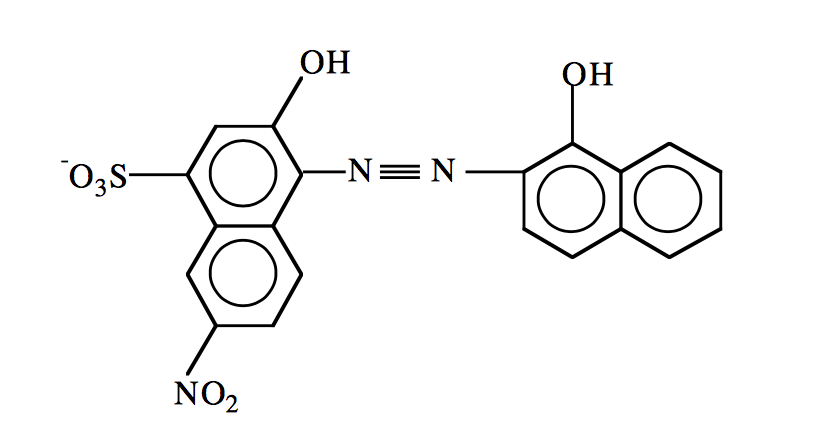
\includegraphics[scale=0.5]{EBT}
        \captionof{figure}{Structure of Eriochrome Black T.}
\end{center}

This weak acid, denoted as H$_2$In$^-$ in Equation 4, changes from a
blue color to purple-red when complexed with a metal ion, denoted as M in
Equations 4 and 5.  EDTA is a stronger complexing ligand than EBT, and therefore
will displace the indicator from the metal ion, returning the indicator to its
original, uncomplexed color of blue, as indicated in Equation 5. \cite{mtsu}
\begin{center} 
\begin{align}
        \ce {M^2+ + $\underset{\mathrm{blue}}{\ce{H_2In^-}}$ + 2H2O 
        &<=> $\underset{\mathrm{purple-red}}{\ce{MIn^-}}$ + 2H3O^+}\\ 
        \ce {$\underset{\mathrm{purple-red}}{\ce{MIn-}}$ + H^+ + Y^4- 
        &<=> $\underset{\mathrm{blue}}{\ce{MY^2-}}$ + HIn^2-} 
\end{align} 
\end{center}

To facilitate the complexation reaction, the solution is kept basic at a pH of
around 10. Table 4 shows the different pK$_a$ values of EBT. \cite{chemwiki}
\begin{center}
        \captionof{table}{Different pK$_a$ values of EBT.}
        \begin{tabular}{|c|c|c|}
                \hline
                & pK$_{a1}$ & pK$_{a2}$ \\
                \hline
                Values: & 6.2 & 11.55 \\
                \hline
        \end{tabular}
\end{center}

Figure 5 illustrates the color changes that EBT undergoes from being complexed
with a metal ion.

\begin{center}
        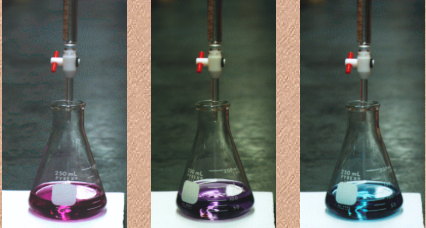
\includegraphics[scale=0.5]{EBT_color}
        \captionof{figure}{Color changes that EBT undergoes during complexation
        reactions. EBT is purple-red when complexed with a metal ion, and blue
        when uncomplexed.\cite{IUS}}
\end{center}

Calcium ion does not form a stable complex with EBT, therefore a titration of Ca$^{2+}$ by EDTA may
not cause a distinctive color change from the EBT indicator at the end point.
The magnesium ion however does form a stable complex with EBT.

The K$_f$ of Mg$^{2+}$ with EDTA is lower than the K$_f$ of Ca$^{2+}$ with
EDTA. Therefore, the total number of moles of Ca$^{2+}$ and Mg$^{2+}$ in a solution
can be determined from a displacement titration using EDTA, where the endpoint
observed is when the EDTA extracts the Mg$^{2+}$ ions from EBT.

To aid in this displacement titration by ensuring that there is some magnesium
present in the sample to be titrated, a small amount of Mg-EDTA is added with
the EDTA solution.

\subsubsection {Murexide}

Murexide (C$_8$H$_8$N$_6$O$_6$), like Eriochrome Black T, is a metallochromic indicator that can be
used in the determination of water hardness. Murexide, when complexed with calcium, turns pink at pH
levels of 12 and higher. At this pH, magnesium precipitates as Mg(OH)$_2$. Therefore, the amount of
Ca$^{2+}$ ions in solution can be determined using Murexide as an indicator. \cite{wroclaw} 
When titrated with EDTA, murexide is displaced from its complexation with Ca$^{2+}$ and turns
blue-purple, and the endpoint is observed.

Figure 6 illustrates the structure of murexide.\cite{murexide}
\begin{center}
        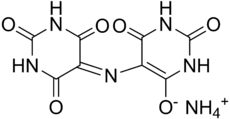
\includegraphics[scale=0.8]{murexide}
        \captionof{figure}{Structure of murexide.}
\end{center}

These complexometric reactions can be followed from Equations 6 and 7, where H$_2$In$^-$ is the
indicator, M is the metal ion, and Y is EDTA.
\begin{center} 
\begin{align}
        \ce {M^2+ + $\underset{\mathrm{blue-purple}}{\ce{H_2In^-}}$ + 2H2O 
        &<=> $\underset{\mathrm{pink}}{\ce{MIn^-}}$ + 2H3O^+}\\ 
        \ce {$\underset{\mathrm{pink}}{\ce{MIn-}}$ + H^+ + Y^4- 
        &<=> $\underset{\mathrm{blue-purple}}{\ce{MY^2-}}$ + HIn^2-} 
\end{align} 
\end{center}

Table 5 shows the different pK$_a$ values of murexide. \cite{dojindo}
\begin{center}
        \captionof{table}{Different pK$_a$ values of murexide.}
        \begin{tabular}{|c|c|c|c|}
                \hline
                & pK$_{a1}$ & pK$_{a2}$ & pK$_{a3}$ \\
                \hline
                Values: & 0 & 9.2 & 10.5 \\
                \hline
        \end{tabular}
\end{center}


\subsection {Masking Agent}
There are often cases where multiple different metal ions exist in a sample to
be analyzed. Other metal ions, such as nickel, can interfere with the
complexometric titration of Ca$^{2+}$ and Mg$^{2+}$ using EDTA and Eriochrome
Black T. Such ions in solution can cause indistintive endpoints, or may bind
more preferentially with either EDTA or EBT than the analytes of interest.

A masking agent is a reagent that can be added to a sample solution to prevent the ions from
binding with EDTA and interfering with analysis.
Common masking agents may include ammonium hydrogen difluoride,
2,3-Dimercapto-1-propanol, and potassium cyanide.


\subsection{Using a Burette}
In a titration, increments of a reagent solution, called the titrant, are added to the analyte until
the reaction has proceeded to completion. The titrant is usually added from a burette, which allows
for an accurate measurement of the volume of titrant added.\cite{Harris}
Figure 7 provides an illustration of a burette.
\begin{center}
        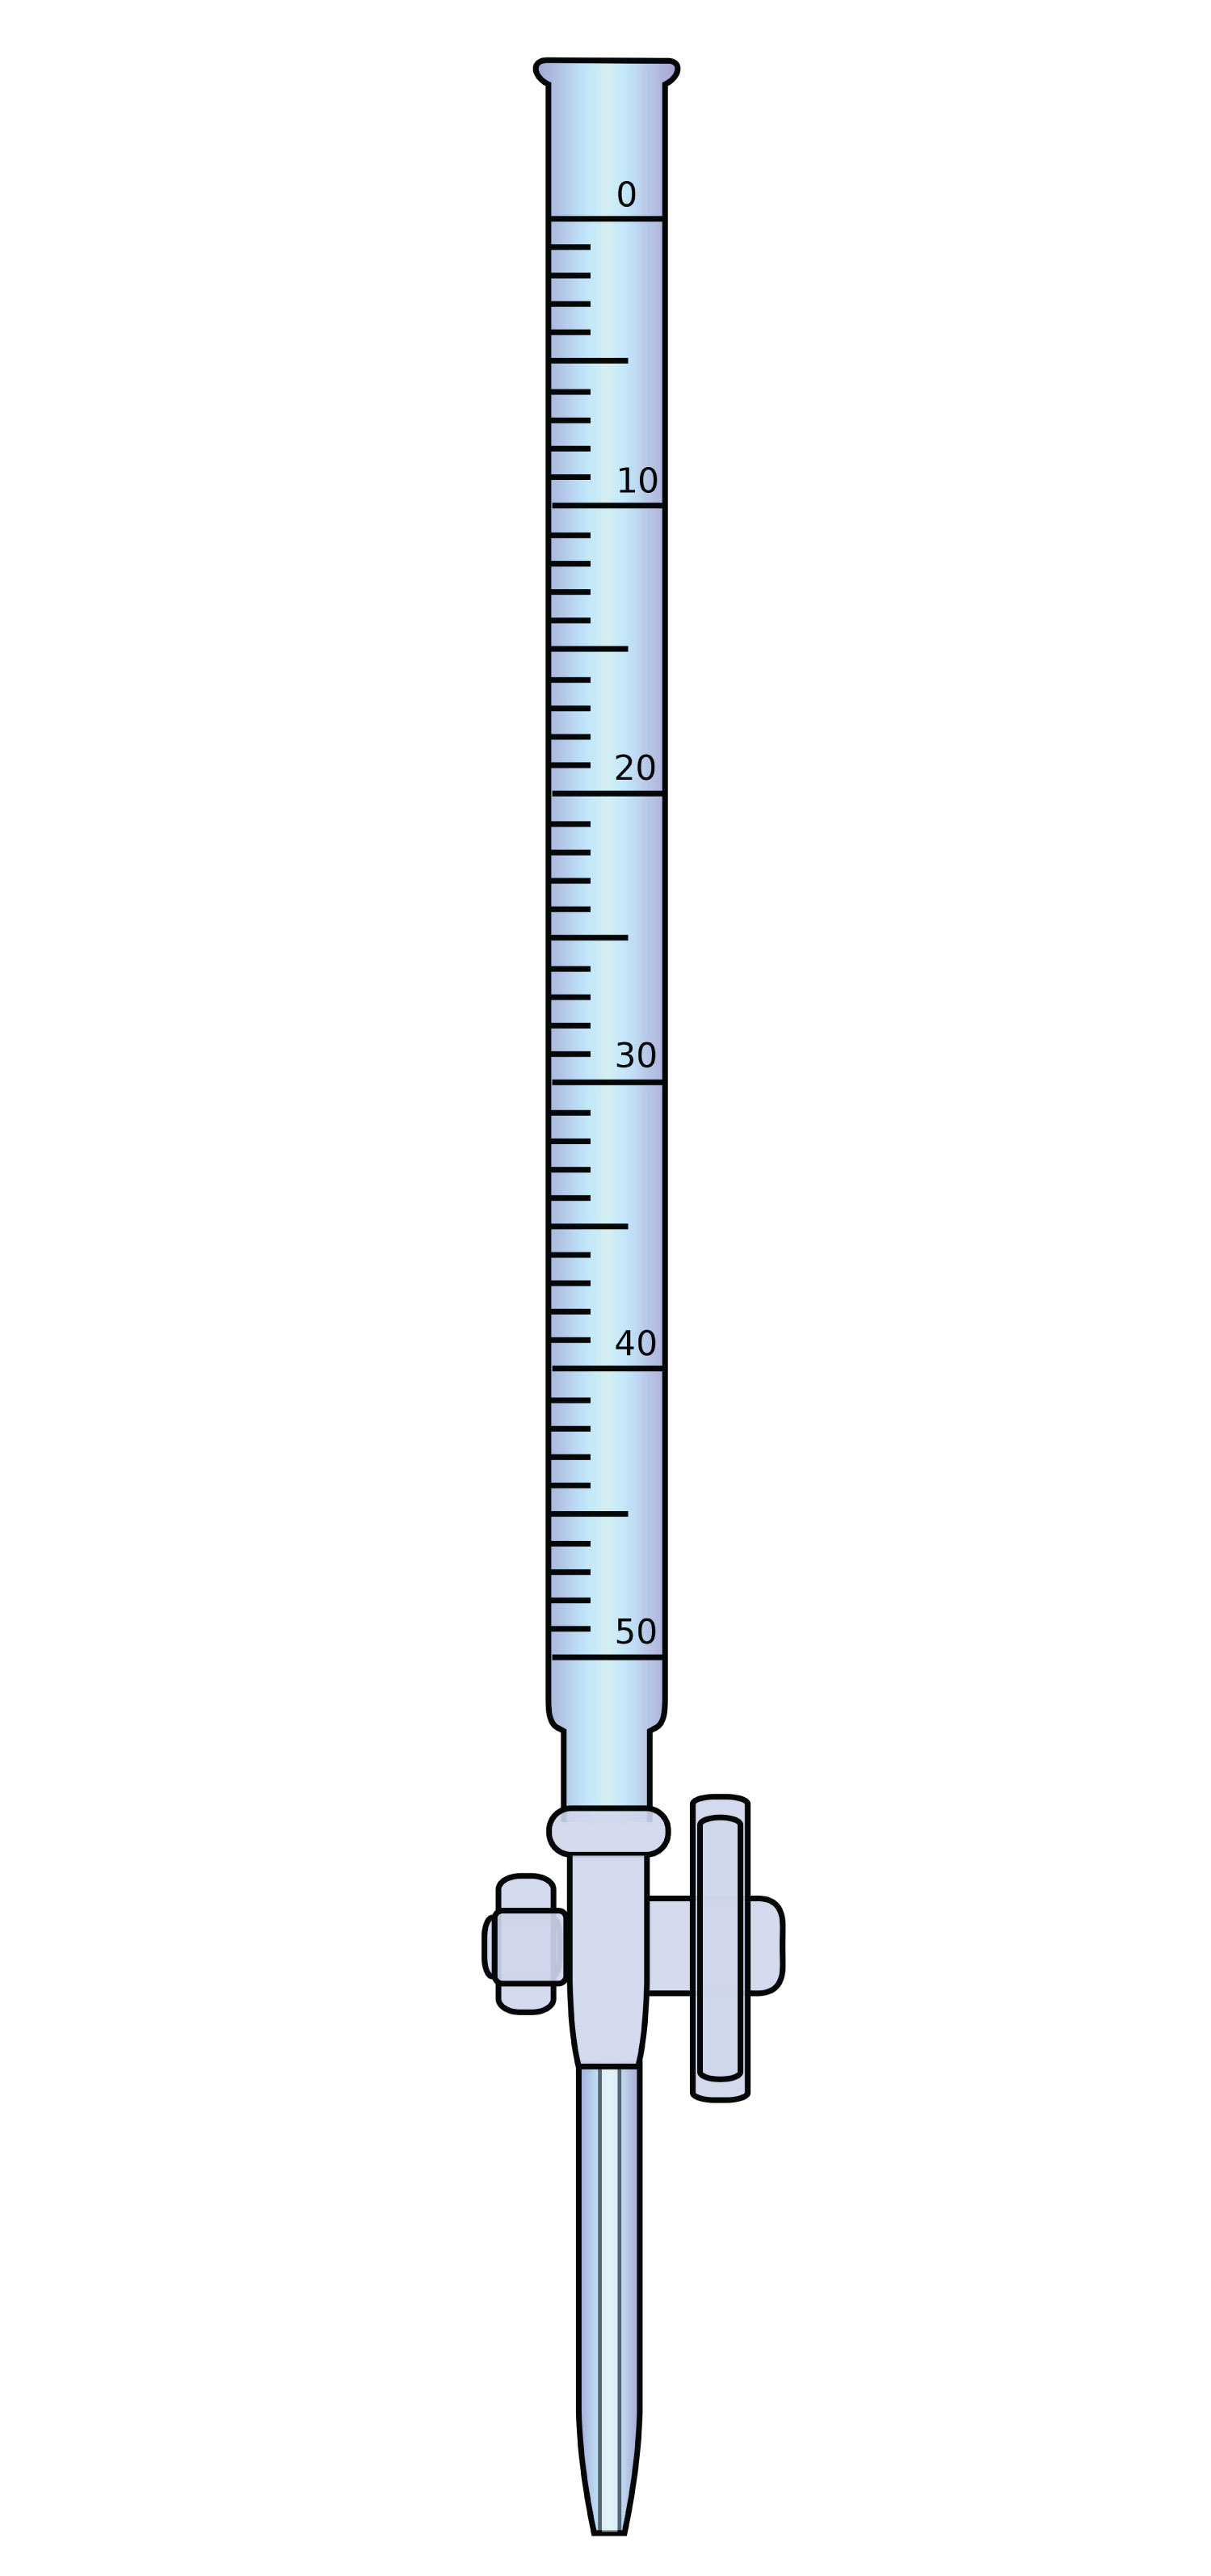
\includegraphics[scale = 0.05]{buret}
        \captionof{figure}{Illustration of burette. \cite{buret}}
\end{center}

The burette is usually glass so that the liquid inside can be observed easily.  The numbers on a
burette are labled with "0" at the top and increasing as they proceed down the side. In this manner,
it is easy to measure the amount of titrant used by subtracting the final volume remaining in the
burette from the initial volume. There is a valve at the bottom of the burette that allows the
titrant to be released ranging from a steady flow to a single drop. Controlling the level of flow is
essential in ensuring that an accurate measurement of titrant needed for the reaction to proceed to
completion is taken.


\section {Results}

Figure 8 illustrates the color changes conducted with Eriochrome Black T as a
reference point in test tubes prior to conducting complexometric titrations.

\begin{figure}[!hb]
\centering
        \begin{subfigure}{.3\textwidth}
        \centering
                \includegraphics[width=.9\linewidth]{tubes_123}
        \end{subfigure}%
        \begin{subfigure}{.3\textwidth}
                \centering
                \includegraphics[width=.9\linewidth]{tubes_456}
        \end{subfigure}%
        \begin{subfigure}{.3\textwidth}
                \centering
                \includegraphics[width=.9\linewidth]{tubes_7}
        \end{subfigure}%
        \caption{Testing of color changes for Eriochrome Black T. Test tubes are
        labeled 1-7 from left to right.}
\end{figure}

Test tubes 1 through 3 demonstrate the pH effects on the Eriochrome Black T
indicator.

Test tube 1 contains EBT, H$_2$O, HCl, and MgCl$_2$.
This test tube demonstrates the EBT in a state of being protonated in acidic
conditions.

Test tube 2 contains EBT, H$_2$O, HCl, NaOH, MgCl$_2$, and a buffer solution of pH 10.
This test tube demonstrates the EBT first being deprotonated as the solution changes
to a basic pH with the addition of NaOH, then becoming more protonated as a pH
10 buffer solution is added.

Test tube 3 contains EBT, H$_2$O, NaOH and MgCl$_2$.
This test tube demonstrates the EBT in a state of being deprotonated in basic
conditions.

Test tubes 4 through 5 demonstrate the Eriochrome Black T indicator complexing
with metals.

Test tube 4 contains EBT, H$_2$O, a buffer solution of pH 10, and EDTA.
This test tube demonstrates the EBT in a state of being deprotonated in basic
conditions.

Test tube 5 contains H$_2$O, a buffer solution of pH 10, EDTA, and
MgCl$_2$.
This test tube demonstrates the conditions where no EBT is in solution.

Test tube 6 contains EBT, H$_2$O, a buffer solution of pH 10, EDTA, and
MgCl$_2$.
This test tube demonstrates the EDTA extracting Mg$^{2+}$ from EBT in a pH 10
buffer solution.

Test tube 7 demonstrates the effects of KCN as a masking agent.
Test tube 7 contains a buffer solution of pH 10, H$_2$O, EBT, NiSO$_4$, EDTA,
and KCN.
As NiSO$_4$ is added to a pH 10 solution containing EBT, the color changes to
purple-red as the EBT complexes with Ni$^{2+}$. No change is observed with EDTA
is added next. As KCN is added to the solution however, KCN inhibits EDTA from
complexing with Ni$^{2+}$ and EBT is allowed to complex again with Ni$^{2+}$.
This should cause the color of the solution to return to blue.

Tables 6 and 7 provide the water hardness results of this experiment. 
The water sample used was sourced from tap water from a sink in the lab.
This lab is located in room WEL 4.124 at The University of Texas at Austin.
The water filter pitcher used in this experiment was Pitcher 3.

Please refer to the Appendix for detailed calculations in determining results and
statistics.

\begin{center}
        \captionof{table}{Water hardness results for unfiltered water.}
        \begin{tabular}{|L|L|L|L|}
                \hline
                \textbf{Concentration of analyte in unknown sample} &
                \textbf{Average \hspace{2cm}$\pm$ Std Dev} & \textbf{\%RSD} &
                \textbf{Average $\pm$ 90\% confidence interval} \\
                \hline
                Total hardness (ppm CaCO$_3$) & 66.2 $\pm$ 1.34 ppm & 2.02\% &
                66.2 $\pm$ 2.26 ppm \\
                \hline
                Calcium hardness (ppm Ca$^{2+}$) & 10.3 $\pm$ 0.213 ppm & - & -
                \\
                \hline
                Magnesium hardness \hspace{2cm} (ppm Mg$^{2+}$) & 9.86 $\pm$ 0.196 ppm & - &
                - \\
                \hline
        \end{tabular}
\end{center}


\begin{center}
        \captionof{table}{Water hardness results for filtered water.}
        \begin{tabular}{|L|L|L|L|}
                \hline
                \textbf{Concentration of analyte in unknown sample} &
                \textbf{Average \hspace{2cm}$\pm$ Std Dev} & \textbf{\%RSD} &
                \textbf{Average $\pm$ 90\% confidence interval} \\
                \hline
                Total hardness (ppm CaCO$_3$) & 28.1 $\pm$ 1.20 ppm & 4.27\% &
                28.1 $\pm$ 2.02 ppm \\
                \hline
                Calcium hardness (ppm Ca$^{2+}$) & 1.74 $\pm$ 0.269 ppm & - & - \\
                \hline
                Magnesium hardness \hspace{2cm} (ppm Mg$^{2+}$) & 5.78 $\pm$
                0.128 ppm & - & - \\
                \hline
        \end{tabular}
\end{center}

\section {Discussion}
It should be noted that the preparation of the EDTA solution was not done via a
weigh-by-difference technique. Therefore, systematic error may be present in the
calculation of the concentration of EDTA used in this experiment. Random error
is always a factor in the preparation of glassware, reagents, and in the
conduction of reactions.

\subsection {Analysis of Test Tube Reactions}
The reactions conducted in the test tubes were to done to study the effects of
EBT under various conditions, as well as to simulate the effects of a masking
agent. Test tubes 1, 3, 4, and 5 reacted as expected and the expected colors
of pink-red, orange-red, blue, and colorless respectively, were produced.

Test tube 2 resulted in a blue solution at the bottom and a red solution on top.
This is likely due to an inadequate mixing of all the reagents in solution. The
pH 10 buffer solution added afterwards likely remained near the top of the test
tube and was not adequately mixed to reach the bottom half of the solution.

Test tube 6 exhibits a clear solution near the bottom and a red solution on top.
The expected outcome is a blue solution overall. This is likely also do an
inadequate mixing of all reagents in solution. Additionally, this test tube must
contain foreign protons that might be protonating the EBT. This would explain a
colorered state of red, which indicates a protonated EBT as depicted in test
tube 1.

Test tube 7 remains in a colored state of red, where as the expected result is
a colored state of blue. It is possible that the masking reagent KCN reacts in
kinetically slow manner, and given sufficient time, would eventually cause the
solution to turn blue. Other reasons may also include foreign elements in the
solution such as residual Na protons from the disodium EDTA salt, which may be
causing the EBT to remain in a state of protonation as consistent with what is
seen in test tube 1.

All these errors are deviations in accuracy, as compared with
literature. \cite{lab_man} These sources of error may be categorized as gross
error, and can be remedied in a number of ways. One remedy is to ensure that all
test tubes have been thoroughly acid washed and dried, preferably in an oven,
prior to conducting these tests. This would help eliminate the presence of
foreign elements. It would also be helpful to ensure that all reagents used have
not been contaminated or have degraded in any way.


\subsection {Analysis of Water Hardness Results}

The average total water hardness for unfiltered water was found to be 66.2 $\pm$
1.34 ppm. According to the US Geological Survey, this is categorized as
"moderately hard". 
The low \%RSD value of 2.02\% and 90\% confidence interval of $\pm$ 2.26 ppm show an
acceptable level of precision in the results
The level of calcium hardness is calculated to be 10.3 $\pm$ 0.213 ppm.
The level of magnesium hardness is calculated to be 9.86 $\pm$ 0.196 ppm.

The average total water hardness for filtered water was found to be 28.1 $\pm$ 1.20 ppm. According
to the US Geological Survey, this is categorized as "soft".
The low \%RSD value of 4.27\% and 90\% confidence interval of $\pm$ 2.02 ppm show an
acceptable level of precision in the results
The level of calcium hardness is calculated to be 1.74 $\pm$ 0.269 ppm.
The level of magnesium hardness is calculated to be 5.78 $\pm$ 0.128 ppm.

This 57.6\% reduction in total water hardness is a testament to the filtering
system employed by Brita\textsuperscript{\textregistered}.
It would appear that the Brita\textsuperscript{\textregistered} filter system
filters out calcium more efficiently than magnesium, as there is a 83.1\%
reduction in calcium levels as compared to a 41.4\% reduction in magnesium
levels.

According to the City of Austin August, 2016 monthly report on water quality,
there is on average a 72 ppm level of water hardness with a minimum of 65 ppm
and maximum of 76 ppm. This testing was conducted at the Davis Water Treatment
Plant.\cite{austin} The unfiltered water hardness levels found in this
experiment are lower than those reported by the City of Austin. This deviation
of accuracy may be because the water sourced from the lab comes from a different
source than the Davis Water Treatment Plant. Furthermore, The University of
Texas at Austin may be responsible for additional treatments of its water.

The accuracy of the filtered water sample was unable to be evaluated due to a
lack of reference in literature.

Sources of error may include systematic errors in the way findings were
calculated, as different burettes were used in the titrations of all samples. 
Human error is always possible, and may be even more prevalent since multiple
different people conducted titrations accross all the samples. Other systematic
errors may include inconsistent determinations of endpoint from color changes
observed by the indicator. One person's definition of a color shade and level
will differ from another's, and can result in unequal reports of endpoints in
titrations. This issue can be addressed by either having only one person conduct
all titrations in the experiment to keep the standards consistent, or have an
average taken from a larger sample set of titrations done by different people.

At any pH, a mass balance on EDTA requires that the total concentration must
equal all of the combined concentrations of each of the forms that EDTA can
have. This is illustrated in Equation 8.
\begin{align}
        \ce {C_{EDTA} = [H6Y^{2+}] + [H5Y+] + [H4Y] + [H3Y^{-}] + [H2Y^{2-}] +
        [HY^{3-}] + [Y^{4-}]}
\end{align}
This means that even at a pH of around 10, there are other forms of EDTA present
in solution. As mentioned earlier, only the Y$^{4-}$ ion complexes in a 1:1
ratio with metal ions. Therefore, there can be expected a lower number of Y$^{4-}$
ions present in a given solution than what is actually used in calculating the
moles of EDTA that react to complex with the metal ions.\cite{chemwiki} This is even more so
the case given the pK$_{a6}$ value of EDTA is 10.37. These conclusions mean that
the reported levels of water hardness may be higher than the actual levels of
the sample.
This same concept applies to the Eriochrome Black T and Murexide indicators as
well.

In this experiment, a buffer solution was used to keep the pH at around 10. This
solution consisted of ammonia/ammonium chloride.
Ammonia may form several stable M$^{2+}$-NH$_3$ complexes, where M = Ca or Mg.
EDTA does form a stronger complex with Ca$^{2+}$ and Mg$^{2+}$ and will
eventually displace NH$_3$, but the overall stability for the M-EDTA complex
will decrease in solution. The effects of such an auxiliary complexing agent may
cause the reported levels of water hardness to be higher than the actual levels
of the sample.

\newpage
\section {Conclusion}

The results of this experiment are reasonable and are deemed to be reproducible
given the same water sources and reagents for testing.
Both the unfiltered water results found in this experiment and the levels of
water hardness reported by the City of Austin fall within the "moderately hard"
category given by the US Geological Survey, and show a level of accuracy and
precision in the results obtained in this experiment.
The filtered water sample is found to be "soft" according to USGS, and
demonstrate the effectiveness of a Brita\textsuperscript{\textregistered}
filtering system on water hardness.

Major sources of error include the assumptions made in calculating the moles of
EDTA that react in a stoichiometric 1:1 ratio. These assumptions ignore the
existence of other species of EDTA present in solution, as well as the presence
and effect of auxiliary complexing agents such as NH$_3$. These sources of error
may cause the reported levels of water hardness in this experiment to be higher
than actual levels.

Additional areas of interest may include the testing of water hardness in
different areas of the City of Austin to see if the findings are consistent with
what is reported. These tests may also reveal patterns in water hardness levels
resultant of geological factors, industrial processes, etc.


\newpage
\bibliographystyle{unsrt}

\bibliography{EDTA.bib}
\newpage


\section*{Appendix}

\begin{enumerate}
        \item Lab notebook pages with raw data and calculations.
\end{enumerate}


\end {document}
